% !TeX encoding = UTF-8
% !TeX root = MAIN.tex

\chapter{Motivation}


The starting point of this thesis is recently conducted research which studies the link and causal effects between monetary policy decisions by the FED and stock market in the U.S.  not only in an ex-post,  but moreover in an ex-ante sense.

The paper "Stock Returns over the FOMC Cycle" \parencite{cieslak_stock_2019} finds that "the equity premium is entirely earned in even weeks starting from the last FOMC meeting (0,  2,  4 and 6)" which implies that the FED has "overly affected the stock market via unexpectatly accommodating policy". 

Another paper "The Economics of the FED Put"  \parencite{cieslak_economics_2020} uses textual analysis of FOMC scripts to identify and measure the causal effect that policy makers indeed pay intention to the "stock market" and negative stock returns are linked with downgrades in growth projections (in an ex-post sense) since the mid-1990s.  
Although policy makers seem to be aware of that the so-called "FED put" "could induce risk-taking" the paper concludes that it does not "significantly affect their decision-making in an ex-ante sense".

TODO: Add thesis goal/Purpose statement..


\chapter{What is the "Fed Put" and how can it be explained?}


TODO: Rewrite 


\chapter{Does the stylized fact of stock excess returns are mainly achieved in FOMC even weeks (0,  2,  4,  6) from 2016 onwards still persist?}



Empirical part I

TODO: Explain how the FOMC cycle time is defined.

TODO: Explain the one of the main regression models used in the paper "Stock Returns over the FOMC Cycle" \parencite{cieslak_stock_2019}

\begin{equation}
	rx_{i}=\hat{\beta_{0}}+D_0*\hat{\gamma_{1}}+D_1*\hat{\gamma_{2}}+\epsilon_i
\end{equation}
where
\begin{equation}
    D_0=
    \begin{cases}
      1, & \text{if in the 0 week within FOMC cycle time. }\\
      0, & \text{otherwise}
    \end{cases}
\end{equation}
and
\begin{equation}
    D_1=
    \begin{cases}
      1, & \text{if in the 2,4 or 6 week within FOMC cycle time. } \\
      0, & \text{otherwise}
    \end{cases}
\end{equation}


Interpret regression results in  \parencite{cieslak_stock_2019}

Line340 replication code add:
"esttab using "Out.tex", stats(N) b(a3) starlevels(*  0.10 ** 0.05 *** 0.010) label nogaps nonote"

{


\ref{table_cies19_1}
\begin{table}
\begin{center}
\begin{adjustbox}{width=1\textwidth}
%%% estout toutput:
\def\sym#1{\ifmmode^{#1}\else\(^{#1}\)\fi}
\begin{tabular}{l*{3}{c}}

\hline\hline
                    &\multicolumn{1}{c}{(1)}&\multicolumn{1}{c}{(2)}&\multicolumn{1}{c}{(3)}\\
                    &\multicolumn{1}{c}{1-day excess return, day t, pct}&\multicolumn{1}{c}{1-day excess return, day t, pct}&\multicolumn{1}{c}{1-day excess return, day t, pct}\\
\hline
Dummy=1 in Week 0   &       0.174*  &       0.136***&      0.0754*  \\
                    &      (1.92)   &      (2.76)   &      (1.78)   \\
Dummy=1 in Week 2,4,6&       0.176***&      0.0993***&      0.0674*  \\
                    &      (2.67)   &      (2.65)   &      (1.68)   \\
Constant            &     -0.0488   &     -0.0210   &     0.00401   \\
                    &     (-1.15)   &     (-0.96)   &      (0.19)   \\
\hline
N                   &         783   &        5214   &        2937   \\
\hline\hline

\end{tabular}
%%%
\end{adjustbox}
\caption{\label{table_cies19_1}TODO: add a caption here.}
\end{center}
\end{table}

}




TODO: Use the regression model to estimate variable for a newer timeframe from 2016 onwards.

\chapter{Is there empirical evidence for a similar effect when considering only the euro-zone and euro-zone stock returns.  Does it imply an equivalent of the Fed Put in the Euro-Zone?}

Empirical part II

Substitute for euro-zone stock excess returns as regressor variable.

Also regress on "ECB policy meetings calendar week". 

* Can anything be learned/infered from the new regressions? -> Probably not really.
* Low R2, missing controls/covariates, missing domain specific knowledge, etc.
* causal mechanism?
* How much do 2 specific events excluded from the results change the regression results?
* Any implications???


\begin{figure}[h]
    \centering
    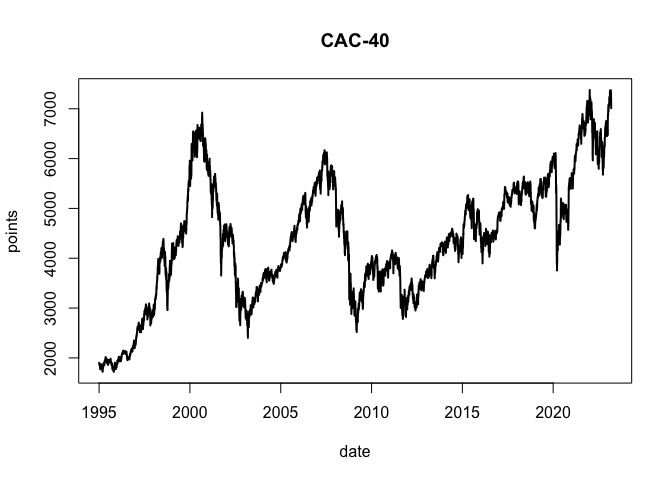
\includegraphics[width=0.9\textwidth]{figures/cac-40}
    \caption{CAC-40 Index from 3rd january 1995 to 27th march 2023}
\end{figure}

\chapter{Conclusion}

Conclusio


